\documentclass[../manuale-utente.tex]{subfiles}

\begin{document}

\subsection{Requisiti}%
\label{sub:requisiti}

\begin{description}
    \item[Sistema operativo:] Android 5.0 o superiore.
    \item[Processore:] ARM32, ARM64, x86, x86\_64.
    \item[Geolocalizzazione:] A-GPS obbligatorio, Glonass e Galileo consigliati.
    \item[Sensori:] Giroscopio, Accelerometro.
\end{description}
\newpage

\subsection{Manuale d'uso}%
\label{sub:manuale_uso_mobile}

\subsubsection{Pagina di accesso}%
\label{sub:pagina_di_accesso}

\begin{figure}[H]
    \centering
    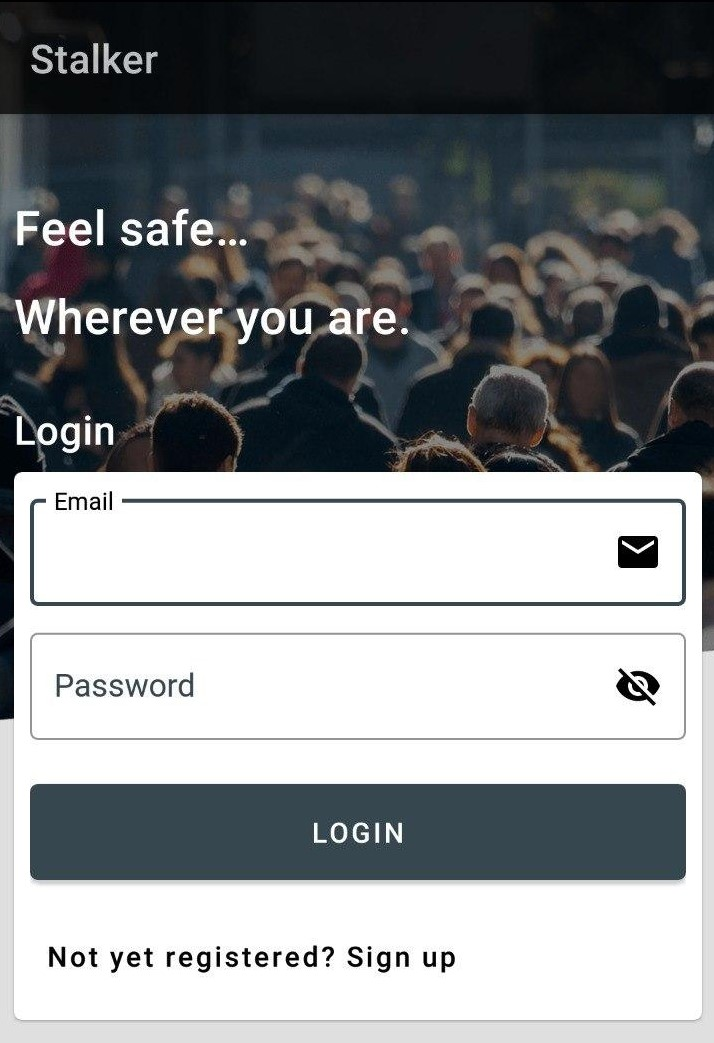
\includegraphics[width=70mm]{img/mobile-app/pagina-di-accesso.jpg}
    \caption{Pagina di accesso}%
    \label{fig:mobile_app_pagina_di_accesso}
\end{figure}

Al primo avvio di Stalker app, l'utente visualizza la pagina di login. 
Per accedere al servizio l'utente dovrà seguire questi tre passaggi:
\begin{itemize}
    \item inserire correttamente l'email.
    \item inserire la password, e possibilmente visualizzarla durante la sua digitazione cliccando sulla figura a fine riga, che deve contenere almeno 8 caratteri alfanumerici e al massimo ne può contenere 32.
    \item selezionare il pulsante \textbf{Login} per inviare le credenziali al server.
\end{itemize} 

Se i dati inseriti sono corretti allora l'utente potrà entrare e cominciare ad essere monitorato!
In caso contrario, se l'utente inserisce delle credenziali non valide, l'accesso a Stalker sarà per forza negato.\\
Le cause possono essere le seguenti:
\begin{itemize}
    \item l'email inserita non rispetta i vincoli imposti dal sistema di Stalker.
    \item la password non rispetta i vincoli imposti dal sistema di Stalker.
    \item l'email e la password inserite non rispettano i vincoli imposti dal sistema di Stalker.
    \item l'email inserita rispetta i vincoli, ma non è presente all'interno del database di Stalker.
    \item la password inserita rispetta i vincoli, ma non è presente all'interno del database di Stalker.
    \item l'email e la password inserite rispettano i vincoli, ma non sono presenti all'interno del database di Stalker.
\end{itemize}

Se l'utente non possiede delle credenziali, ha la possibilità di registrarsi, grazie all'apposito form disponibile dopo aver cliccato su \textit{Not yet registered? Sign up}.
\newpage

\subsubsection{Pagina di registrazione}%
\label{sub:pagina_di_registrazione}

\begin{figure}[H]
    \centering
    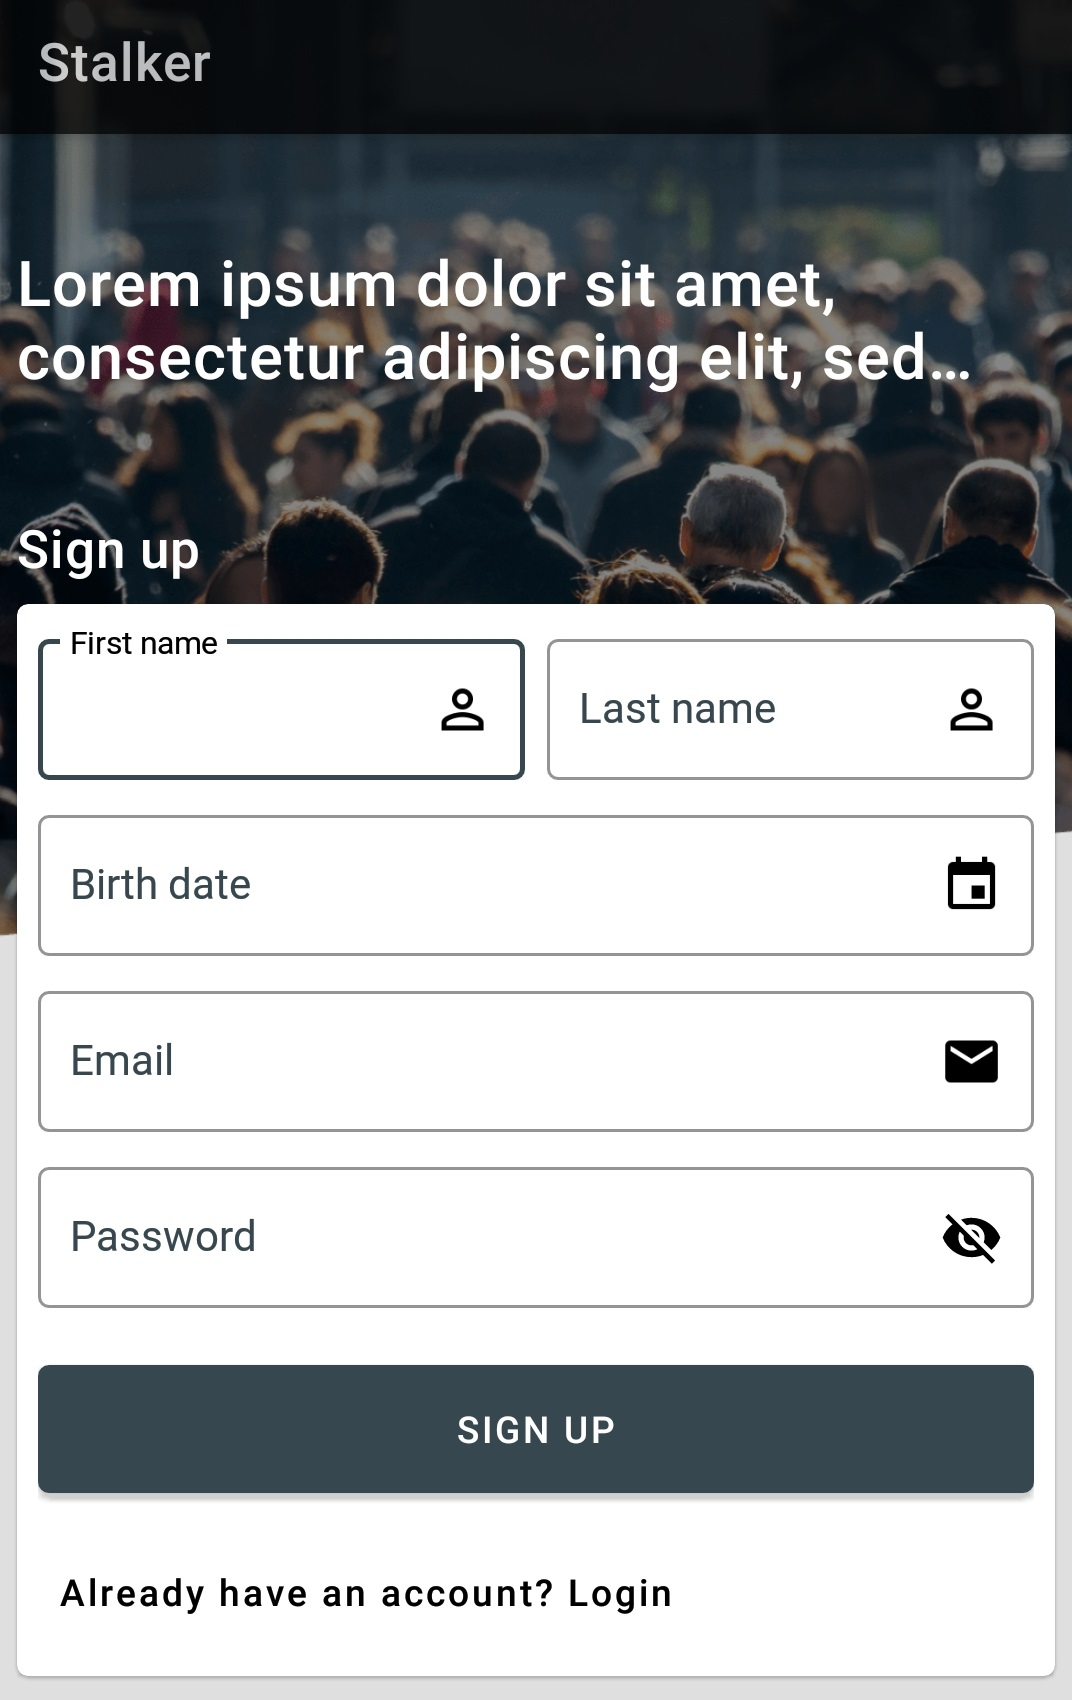
\includegraphics[width=70mm]{img/mobile-app/pagina-di-registrazione.jpg}
    \caption{Pagina di registrazione}%
    \label{fig:mobile_app_pagina_di_registrazione}
\end{figure}

Se l'utente non si è mai registrato in Stalker, questo form è l'unico modo per farlo!\\
L'utente per registrarsi deve inserire delle semplici informazioni personali:

\begin{itemize}
    \item inserire il nome.
    \item inserire il cognome.
    \item inserire la data di nascita.
    \item inserire l'email, non precedentemente utilizzata in Stalker.
    \item inserire la password, che deve essere alfanumerica con almeno 8 caratteri e al massimo 32.
    \item premere il pulsante sign up per effettuare la registrazione.
\end{itemize}

Si avvisa inoltre che non è possibile registrarsi più volte con la stessa email.\\
Se questi vincoli non saranno rispettati l'utente non potrà registrarsi.\\
Se l'utente possiede delle credenziali, ha la possibilità di accedere, grazie all'apposito form disponibile dopo aver cliccato su \textit{Already have an account? Login}.
\newpage

\subsubsection{Pagina iniziale}%
\label{sub:pagina_iniziale}

% \begin{figure}[H]
%     \centering
%     \includegraphics{img/mobile-app/pagina-iniziale.png}
%     \caption{Pagina iniziale}%
%     \label{fig:mobile_app_pagina_iniziale}
% \end{figure}

Lorem ipsum

% add other functionalities 

\end{document}